% ======================================================================
%  Chapter 4 — Periodic Media and Photonic Bands
% ======================================================================

\section{Periodicity in optics}
\label{sec:ch4-periodicity}

A photonic crystal is a medium whose material matrix is periodic:
\begin{equation}\label{eq:ch4-periodicity}
  \Mmat(\rvec + \avec_i) = \Mmat(\rvec)
  \qquad\text{for lattice vectors } \avec_1, \avec_2, \avec_3\,.
\end{equation}
In two dimensions, the periodicity is in the $(\avec_1,\avec_2)$ plane
and $\Mmat$ is independent of $z$ (or periodic with a different period
in $z$); in one dimension, a single $\avec_1$ suffices.  This chapter
focuses on the two-dimensional case, which is the most important for
topological photonics, but the formalism applies in any dimension.

The physical origin of the periodicity can be a lattice of dielectric
rods, a pattern of holes in a slab, a structured metallic or ferrite
arrangement, or any other design in which the optical properties repeat.
What matters for the mathematics is only the discrete translational
symmetry \eqref{eq:ch4-periodicity}.

\section{Bloch's theorem for Maxwell modes}
\label{sec:ch4-bloch}

\subsection{Statement and proof}
\label{sec:ch4-bloch-statement}

\begin{theorem}[Bloch's theorem for electromagnetic fields]
  \label{thm:ch4-bloch}
  Let $\Mmat(\rvec)$ be periodic with lattice vectors $\{\avec_i\}$.
  Then every eigenmode of the Maxwell operator can be written in the
  Bloch form
  \begin{equation}\label{eq:ch4-bloch-form}
    \emfield_{n\kvec}(\rvec)
    = \ee^{\ii\kvec\cdot\rvec}\,\mathbf{u}_{n\kvec}(\rvec)\,,
  \end{equation}
  where $\kvec$ is the Bloch wavevector, $n$ is the band index, and
  $\mathbf{u}_{n\kvec}(\rvec)$ is cell-periodic:
  \begin{equation}\label{eq:ch4-cell-periodic}
    \mathbf{u}_{n\kvec}(\rvec+\avec_i)
    = \mathbf{u}_{n\kvec}(\rvec)
    \qquad\text{for all lattice vectors } \avec_i\,.
  \end{equation}
\end{theorem}

\begin{proof}
Define the translation operator $T_\avec$ by
$(T_\avec\emfield)(\rvec)=\emfield(\rvec+\avec)$.  Since
$\Mmat(\rvec+\avec)=\Mmat(\rvec)$, the Maxwell operator
$\Hamop(\rvec)=\Mmat^{-1}(\rvec)\Maxop$ commutes with $T_\avec$:
\begin{equation}
  [T_\avec,\,\Hamop] = 0
  \qquad\text{for all lattice vectors } \avec\,.
\end{equation}
The translation operators for different lattice vectors also commute
among themselves.  Therefore $\Hamop$ and $\{T_\avec\}$ can be
simultaneously diagonalised.

The eigenvalues of $T_\avec$ on a square-integrable (or Bloch-periodic)
function space are of the form
$T_\avec\emfield=\ee^{\ii\kvec\cdot\avec}\emfield$,
parametrised by a wavevector $\kvec$.  This is because $T_\avec$ is
unitary and the group of translations is Abelian, so its irreducible
representations are one-dimensional and given by characters
$\avec\mapsto\ee^{\ii\kvec\cdot\avec}$.

A simultaneous eigenfunction of $\Hamop$ and $T_\avec$ therefore
satisfies $\emfield(\rvec+\avec)=\ee^{\ii\kvec\cdot\avec}\emfield(\rvec)$.
Writing $\emfield(\rvec)=\ee^{\ii\kvec\cdot\rvec}\mathbf{u}(\rvec)$,
this condition becomes $\mathbf{u}(\rvec+\avec)=\mathbf{u}(\rvec)$:
$\mathbf{u}$ is cell-periodic.
\end{proof}

\subsection{The Brillouin zone}
\label{sec:ch4-bz}

The Bloch wavevector $\kvec$ is defined modulo reciprocal lattice
vectors $\Gvec$
\cite{initio2026pdf}.  Two wavevectors $\kvec$ and $\kvec+\Gvec$ label the
same physical mode (with a different choice of cell-periodic part), so
$\kvec$ can be restricted to a fundamental domain of the reciprocal
lattice---the \emph{first Brillouin zone} $\BZ$.

For a two-dimensional square lattice with period $a$, the reciprocal
lattice vectors are $\Gvec=\frac{2\pi}{a}(m_1\hat{x}+m_2\hat{y})$ and
the Brillouin zone is the square
$|k_x|,|k_y|\leq\pi/a$.  For a hexagonal lattice (which will be
central to the Dirac-cone physics of \chref{ch:dirac-cones}), the
Brillouin zone is a regular hexagon.

\begin{remark}[Topology of the Brillouin zone]
  The identification $\kvec\sim\kvec+\Gvec$ means that the Brillouin
  zone is topologically a \emph{torus} $T^2$ in two dimensions (or
  $T^3$ in three).  This closed, boundary-free topology is essential
  for the quantisation of the Chern number: the integral of the Berry
  curvature over a torus is always an integer multiple of $2\pi$
  (\chref{ch:geometry-bands}).
\end{remark}

\section{The cell-periodic eigenvalue problem}
\label{sec:ch4-cell-evp}

Substituting the Bloch form \eqref{eq:ch4-bloch-form} into the Maxwell
eigenvalue equation $\Maxop\emfield=\omega\Mmat\emfield$ and noting
that $\nabla(\ee^{\ii\kvec\cdot\rvec}\mathbf{u})
=\ee^{\ii\kvec\cdot\rvec}(\nabla+\ii\kvec)\mathbf{u}$, we obtain the
\emph{cell-periodic eigenvalue problem}:
\begin{equation}\label{eq:ch4-cell-evp}
  \boxed{%
  \Maxop(\kvec)\,\mathbf{u}_{n\kvec}(\rvec)
  = \omega_{n\kvec}\,\Mmat(\rvec)\,\mathbf{u}_{n\kvec}(\rvec)\,,}
\end{equation}
where the $\kvec$-dependent curl operator is
\begin{equation}\label{eq:ch4-maxop-k}
  \Maxop(\kvec) =
  \begin{pmatrix}
    \mathbf{0} & \ii(\nabla+\ii\kvec)\times \\[2pt]
    -\ii(\nabla+\ii\kvec)\times & \mathbf{0}
  \end{pmatrix}.
\end{equation}
This operator acts on cell-periodic functions and is parametrised by
$\kvec$.

The inner product for \eqref{eq:ch4-cell-evp} is the electromagnetic
inner product restricted to one unit cell $\Omega$:
\begin{equation}\label{eq:ch4-cell-ip}
  \left\langle \mathbf{u}_1,\mathbf{u}_2\right\rangle_{\Mmat,\Omega}
  = \int_\Omega
  \mathbf{u}_1^\dagger(\rvec)\,\Mmat(\rvec)\,
  \mathbf{u}_2(\rvec)\,\dd^d r\,.
\end{equation}
By the self-adjointness of $\Maxop(\kvec)$ under periodic boundary
conditions (Theorem~\ref{thm:ch3-self-adjoint}), the eigenfrequencies
$\omega_{n\kvec}$ are real and the cell-periodic eigenmodes are
orthogonal:
\begin{equation}\label{eq:ch4-cell-orth}
  \left\langle \mathbf{u}_{n\kvec},\mathbf{u}_{m\kvec}\right\rangle_{\Mmat,\Omega}
  = \delta_{nm}\,.
\end{equation}

\section{Band structure}
\label{sec:ch4-bands}

For each $\kvec$ in the Brillouin zone, the cell-periodic eigenvalue
problem \eqref{eq:ch4-cell-evp} has a discrete set of eigenfrequencies
\begin{equation}
  0 < \omega_{1\kvec} \leq \omega_{2\kvec} \leq \omega_{3\kvec}
  \leq \cdots\,.
\end{equation}
As $\kvec$ varies continuously over the Brillouin zone, each
$\omega_{n\kvec}$ traces out a continuous curve---the $n$-th
\emph{photonic band}.  The collection of all bands is the
\emph{photonic band structure} \cite{wu2015scheme,paz2019tutorial,ho1990existence}.

\subsection{Band gaps}
\label{sec:ch4-band-gaps}

A \emph{photonic band gap} is a frequency range
$(\omega_{\mathrm{low}},\omega_{\mathrm{high}})$ in which no
eigenfrequency exists for any $\kvec$ in the Brillouin zone:
\begin{equation}
  \max_\kvec\omega_{n\kvec} < \omega_{\mathrm{low}}
  < \omega_{\mathrm{high}}
  < \min_\kvec\omega_{(n+1)\kvec}\,
\end{equation}
The displayed formula above follows the convention and normalisation used in \cite{wang2007reflection}.
The existence and width of band gaps depend on the contrast of
$\Mmat(\rvec)$ between different regions of the unit cell and on the
lattice geometry.  High dielectric contrast and connected
high-$\varepsilon$ regions generally favour wider gaps.

Band gaps are essential for topological photonics: the Chern number of a
set of bands is well defined only when those bands are separated from
all others by gaps.  The topological edge states live inside these
gaps.

\subsection{Group velocity and energy velocity}
\label{sec:ch4-velocity}

The group velocity of the $n$-th band is
\begin{equation}\label{eq:ch4-group-velocity}
  \mathbf{v}_{g,n}(\kvec)
  = \nabla_\kvec\,\omega_{n\kvec}\,
\end{equation}
The displayed formula above follows the convention and normalisation used in \cite{raghu2008analogs}.
This can be evaluated using the Hellmann--Feynman theorem
\cite{haldane2008reflection}.
Differentiating the eigenvalue equation
$\Maxop(\kvec)\mathbf{u}_n=\omega_n\Mmat\mathbf{u}_n$ with respect to
$k_\alpha$ and taking the inner product with $\mathbf{u}_n$:
\begin{equation}\label{eq:ch4-hellmann-feynman}
  \pderiv{\omega_n}{k_\alpha}
  = \frac{
    \displaystyle\int_\Omega\mathbf{u}_n^\dagger\,
    \pderiv{\Maxop(\kvec)}{k_\alpha}\,\mathbf{u}_n\,\dd^d r
  }{
    \displaystyle\int_\Omega\mathbf{u}_n^\dagger\,\Mmat\,
    \mathbf{u}_n\,\dd^d r
  }\,.
\end{equation}
The numerator involves the $k_\alpha$-derivative of $\Maxop(\kvec)$,
which from \eqref{eq:ch4-maxop-k} has the structure of a ``velocity
operator'' coupling $\Efield$ and $\Hfield$ components.

The \emph{energy velocity} is defined as the ratio of time-averaged
Poynting flux to time-averaged energy:
\begin{equation}\label{eq:ch4-energy-velocity}
  \mathbf{v}_E
  = \frac{\int_\Omega\langle\Sfield\rangle\,\dd^d r}
         {\int_\Omega\langle u\rangle\,\dd^d r}\,.
\end{equation}
In a lossless nondispersive medium, one can show that
$\mathbf{v}_g=\mathbf{v}_E$ by combining the Hellmann--Feynman relation
with Poynting's theorem.  In a dispersive medium, the equality
$\mathbf{v}_g=\mathbf{v}_E$ still holds provided the energy density
is computed using the dispersive metric $\Mgmat$.

\section{TE and TM modes in two dimensions}
\label{sec:ch4-te-tm}

For a two-dimensional photonic crystal with $\Mmat$ independent of $z$
and no propagation in the $z$-direction ($k_z=0$), the six-component
eigenproblem separates into two independent scalar problems.

\subsection{TM polarisation}
\label{sec:ch4-tm}

The TM modes have $\Efield=E_z\hat{z}$ and
$\Hfield=(H_x,H_y,0)^T$.  The curl equations reduce to a single
scalar equation for $E_z$:
\begin{equation}\label{eq:ch4-tm-scalar}
  -(\nabla+\ii\kvec_\parallel)\cdot\bigl[
    \mut^{-1}(\rvec)\,(\nabla+\ii\kvec_\parallel)E_z(\rvec)
  \bigr]
  = \frac{\omega^2}{c^2}\,\varepsilon_{zz}(\rvec)\,E_z(\rvec)\,,
\end{equation}
where $\kvec_\parallel=(k_x,k_y)$ and $\mut^{-1}$ is the $2\times 2$
in-plane inverse permeability tensor.

For an isotropic nonmagnetic medium ($\mut=\mathbf{I}$), this
simplifies to the standard TM eigenproblem:
\begin{equation}\label{eq:ch4-tm-simple}
  -(\nabla+\ii\kvec_\parallel)^2 E_z(\rvec)
  = \frac{\omega^2}{c^2}\,\varepsilon(\rvec)\,E_z(\rvec)\,.
\end{equation}

\subsection{TE polarisation}
\label{sec:ch4-te}

The TE modes have $\Hfield=H_z\hat{z}$ and
$\Efield=(E_x,E_y,0)^T$.  The scalar equation is
\begin{equation}\label{eq:ch4-te-scalar}
  -(\nabla+\ii\kvec_\parallel)\cdot\bigl[
    \epst^{-1}(\rvec)\,(\nabla+\ii\kvec_\parallel)H_z(\rvec)
  \bigr]
  = \frac{\omega^2}{c^2}\,\mu_{zz}(\rvec)\,H_z(\rvec)\,.
\end{equation}

\subsection{Gyrotropic media: coupling through off-diagonal terms}
\label{sec:ch4-gyrotropic}

When the permeability tensor has off-diagonal gyrotropic components as
in \eqref{eq:ch2-gyrotropic-mu}, the inverse permeability
\begin{equation}\label{eq:ch4-mu-inv}
  \mut_\perp^{-1}
  = \frac{1}{\mu_\perp^2-\kappa^2}
  \begin{pmatrix}
    \mu_\perp & \ii\kappa \\
    -\ii\kappa & \mu_\perp
  \end{pmatrix}
\end{equation}
introduces first-order spatial derivatives through the off-diagonal
gyrotropic elements.  The correct operator form retains the full
tensor contraction with spatially varying coefficients:
\begin{equation}\label{eq:ch4-tm-gyrotropic}
  -D_i\bigl[(\mu^{-1})_{ij}(\rvec)\,D_j E_z\bigr]
  = \frac{\omega^2}{c^2}\,\varepsilon(\rvec)\,E_z\,,
  \qquad D_i\equiv\partial_i+\ii k_i\,,
\end{equation}
where $i,j\in\{x,y\}$ and summation over repeated indices is implied.
For a uniform gyrotropic medium, the off-diagonal elements of
$(\mu^{-1})_{ij}$ contribute through the commutator
$D_i D_j - D_j D_i=0$ (for constant $\kvec$), so the gyrotropic
coupling vanishes.  The physically important gyrotropic effect arises
from the \emph{spatial variation} of $(\mu^{-1})_{ij}(\rvec)$ at
material interfaces, where the differential operator does not commute
with the position-dependent tensor.  This spatially varying gyrotropic
coupling breaks the symmetry $\kvec\to-\kvec$ and is responsible for
the nonzero Berry curvature analysed in \chref{ch:breaking-tr}.

\begin{remark}
In the gyrotropic case, the TE and TM polarisations are not strictly
decoupled when $\kappa\neq 0$ and the geometry mixes in-plane and
out-of-plane components.  However, for a 2D crystal with
$\epst$ diagonal and $\mut$ of the form
\eqref{eq:ch2-gyrotropic-mu}, the TM and TE sectors remain
exactly separated at $k_z=0$.  This separation is exploited in all the
standard topological photonic-crystal designs.
\end{remark}

\section{The plane-wave expansion}
\label{sec:ch4-pwe}

The most widely used method for computing photonic band structures is
the plane-wave expansion (PWE) \cite{ozawa2018topological,haldane2008possible,initio2026pdf}, in which the cell-periodic fields and
material parameters are expanded in Fourier series over reciprocal
lattice vectors.

\subsection{Fourier expansion of fields and material parameters}
\label{sec:ch4-fourier}

Expand the cell-periodic field in a Fourier series:
\begin{equation}\label{eq:ch4-fourier-field}
  \mathbf{u}_{n\kvec}(\rvec)
  = \sum_\Gvec \hat{\mathbf{u}}_{n\kvec}(\Gvec)\,
    \ee^{\ii\Gvec\cdot\rvec}\,,
\end{equation}
and similarly for the material parameters:
\begin{equation}\label{eq:ch4-fourier-eps}
  \varepsilon(\rvec) = \sum_\Gvec \hat{\varepsilon}(\Gvec)\,
    \ee^{\ii\Gvec\cdot\rvec}\,,
  \qquad
  \mu^{-1}(\rvec) = \sum_\Gvec \widehat{\mu^{-1}}(\Gvec)\,
    \ee^{\ii\Gvec\cdot\rvec}\,.
\end{equation}
The Fourier coefficients are computed from integrals over the unit cell:
\begin{equation}\label{eq:ch4-fourier-coeff}
  \hat{\varepsilon}(\Gvec)
  = \frac{1}{A_\Omega}\int_\Omega
    \varepsilon(\rvec)\,\ee^{-\ii\Gvec\cdot\rvec}\,\dd^2 r\,,
\end{equation}
where $A_\Omega$ is the area of the 2D unit cell.

\subsection{Matrix eigenvalue problem}
\label{sec:ch4-matrix-evp}

Substituting the Fourier expansions into the TM eigenvalue equation
\eqref{eq:ch4-tm-scalar}, the convolution of material parameters and
\begin{equation}\label{eq:ch4-pwe-matrix}
  \sum_{\Gvec'}
  (\kvec+\Gvec)_i\,
  \widehat{(\mu^{-1})_{ij}}(\Gvec-\Gvec')\,
  (\kvec+\Gvec')_j\,\hat{E}_z(\Gvec')
  = \frac{\omega^2}{c^2}\sum_{\Gvec'}
    \hat{\varepsilon}(\Gvec-\Gvec')\,\hat{E}_z(\Gvec')\,,
\end{equation}
where summation over repeated Cartesian indices $i,j\in\{x,y\}$ is
implied.  For a scalar (non-gyrotropic) inverse permeability, the
tensor Fourier coefficient reduces to
$\widehat{(\mu^{-1})_{ij}}(\Gvec)=\widehat{\mu^{-1}}(\Gvec)\,
\delta_{ij}$ and the left-hand side simplifies to
$(\kvec+\Gvec)\cdot(\kvec+\Gvec')\,\widehat{\mu^{-1}}(\Gvec-\Gvec')$.
For gyrotropic media, the off-diagonal Fourier components
$\widehat{(\mu^{-1})_{xy}}$ carry the topological information.
In practice, the Fourier series is truncated to $N_G$ reciprocal
lattice vectors, yielding an $N_G\times N_G$ generalised Hermitian
matrix eigenvalue problem at each $\kvec$ point.  The eigenvalues
$\omega_{n\kvec}^2/c^2$ give the band structure; the eigenvectors give
the mode profiles.
$\omega_{n\kvec}^2/c^2$ give the band structure; the eigenvectors give
the mode profiles.

\begin{remark}[Convergence]
  The PWE converges exponentially fast for smooth material profiles and
  algebraically for discontinuous profiles (e.g.\ circular rods).  For
  the latter, careful treatment of the Fourier factorisation (the
  ``inverse rule'' of Li) is needed to avoid slow convergence \cite{raman2010photonic}.  We
  discuss numerical methods further in \chref{ch:computing-chern} and
  \appref{app:numerical-recipes}.
\end{remark}

\section{Examples of photonic band structures}
\label{sec:ch4-examples}

\subsection{Square lattice of dielectric rods}
\label{sec:ch4-square-rods}

Consider a two-dimensional square lattice (period $a$) of circular
dielectric rods (radius $r$, permittivity $\varepsilon_r$) in air
($\varepsilon=1$), with $\mu=1$ everywhere.  This is the standard
textbook photonic crystal.

For TM polarisation, the lowest bands emerge from the folding of the
free-photon dispersion $\omega=c|\kvec+\Gvec|$ at the Brillouin-zone
boundaries.  When the dielectric contrast $\varepsilon_r/1$ is
sufficiently large ($\varepsilon_r\gtrsim 8$ for $r/a\approx 0.2$), a
\emph{complete TM band gap} opens between the first and second bands.

A representative TM band structure for this system, computed by the
plane-wave expansion method with $\varepsilon_r=12$ and $r/a=0.2$,
shows a complete TM gap between the first and second bands spanning
approximately $15\%$ of the mid-gap frequency.  The gap arises because
the first band concentrates its electric field energy in the
high-permittivity rods, while the second band is forced by
orthogonality to concentrate in the low-permittivity air region,
paying a higher electromagnetic energy cost.  This concentration
mechanism---known as the ``dielectric'' and ``air'' band distinction
in the photonic crystal literature---is the spatial analog of the
bonding/anti-bonding splitting in electronic band theory.

\subsection{Hexagonal lattice and Dirac points}
\label{sec:ch4-hex-dirac}

The hexagonal (triangular) lattice is particularly important for
topological photonics.  At the corners $K$ and $K'$ of the hexagonal
Brillouin zone, the $C_{6v}$ point-group symmetry can enforce
\emph{Dirac-point degeneracies}: pairs of bands that touch linearly,
with a dispersion relation locally resembling that of massless
relativistic fermions:
\begin{equation}\label{eq:ch4-dirac-dispersion}
  \omega_\pm(\kvec) \approx \omega_D \pm v_D|\delta\kvec|\,,
\end{equation}
where $\delta\kvec=\kvec-\kvec_D$ is the displacement from the Dirac
point, $\omega_D$ is the Dirac frequency, and $v_D$ is the Dirac
velocity.

These Dirac points are the starting point for topological gap opening:
when time-reversal symmetry is broken by a gyrotropic perturbation, the
degeneracy is lifted and the resulting gapped bands acquire nonzero
Chern numbers.  This is the subject of Chapters~\ref{ch:dirac-cones}
and \ref{ch:breaking-tr}.

\section{Symmetry and degeneracy}
\label{sec:ch4-symmetry}

The symmetries of the photonic crystal---both spatial (point group,
space group) and non-spatial (time reversal)---constrain the band
structure and the allowed degeneracies.

\subsection{Point-group symmetry}
\label{sec:ch4-point-group}

At high-symmetry points in the Brillouin zone, the little group
(the subgroup of the point group that leaves $\kvec$ invariant) determines
the allowed irreducible representations of the eigenmodes.  Bands that
belong to multi-dimensional representations are degenerate.

For example, at the $\Gamma$ point ($\kvec=\mathbf{0}$) of a
$C_{6v}$-symmetric hexagonal lattice, the modes transform under the
full $C_{6v}$ group and can be labelled by the irreducible
representations $A_1$, $A_2$, $B_1$, $B_2$, $E_1$, $E_2$.  The
two-dimensional representations $E_1$ and $E_2$ correspond to doubly
degenerate modes.

\subsection{Time reversal and the dispersion relation}
\label{sec:ch4-tr-dispersion}

When the medium is time-reversal invariant (reciprocal, $\kappa=0$),
the Bloch eigenfrequencies satisfy
\begin{equation}\label{eq:ch4-tr-symmetry}
  \omega_n(\kvec) = \omega_n(-\kvec)\,.
\end{equation}
This is a direct consequence of the time-reversal symmetry derived in
\secref{sec:ch2-time-reversal}: if $\mathbf{u}_{n\kvec}$ is an
eigenmode at $\kvec$, then $\Top\mathbf{u}_{n\kvec}$ is an eigenmode at
$-\kvec$ with the same frequency.

Breaking time-reversal symmetry ($\kappa\neq 0$) allows
$\omega_n(\kvec)\neq\omega_n(-\kvec)$.  This asymmetry is directly
visible in the band structure as a tilt or splitting at time-reversal-related
points, and it is the physical origin of nonreciprocal wave propagation.

\subsection{Inversion symmetry and band sticking}
\label{sec:ch4-inversion}

When the photonic crystal has inversion symmetry
($\Mmat(-\rvec)=\sigma_z\Mmat(\rvec)\sigma_z$), the eigenfrequencies
satisfy $\omega_n(\kvec)=\omega_n(-\kvec)$ \emph{independently} of
time-reversal symmetry.  The combined effect of inversion and
time-reversal symmetry can force additional degeneracies at
high-symmetry points, which is important for the formation of
Dirac points.

\section{From bands to topology}
\label{sec:ch4-bands-to-topology}

The photonic band structure $\{\omega_n(\kvec)\}$ tells us
\emph{where} light can propagate: inside bands, at the corresponding
frequencies and wavevectors.  But the band structure alone does not tell
the full story.  Two photonic crystals can have identical band
structures---the same frequencies, the same gaps---and yet differ in a
fundamental way that affects their interface physics.

The missing information is the \emph{geometry of the eigenmodes} as
functions of $\kvec$.  As $\kvec$ traverses the Brillouin zone, the
cell-periodic mode $\mathbf{u}_{n\kvec}(\rvec)$ rotates in the
Hilbert space of cell-periodic fields.  The rate and manner of this
rotation are captured by the Berry connection and Berry curvature,
which we derive in the next chapter.

The topological invariant---the Chern number---is an integer that
characterises the \emph{global} geometry of each band over the entire
Brillouin zone \cite{thouless1982quantized}.  It cannot be changed by any smooth deformation of the
medium that does not close the band gap.  When two media with different
Chern numbers are brought together, the mismatch forces the existence
of interface modes that cross the gap: these are the topological edge
states.

\section{Group velocity and the Maxwell Hellmann--Feynman theorem}
\label{sec:ch4-group-velocity}

The group velocity of a Bloch mode is the gradient of the band
frequency with respect to the wavevector:
$\mathbf{v}_g=\nabla_\kvec\omega_n(\kvec)$.  This can be computed
directly from the eigenvalue equation by a Hellmann--Feynman argument.

Differentiating the Bloch eigenproblem
$\Maxop(\kvec)\mathbf{u}_{n\kvec}
=\omega_{n\kvec}\Mmat\mathbf{u}_{n\kvec}$ with respect to $k_a$
and projecting onto $\mathbf{u}_{n\kvec}$ gives
\cite{gangaraj2016berry,ozawa2018topological}
\begin{equation}\label{eq:ch4-hellmann-feynman-group}
  v_{g,a}
  = \frac{\partial\omega_n}{\partial k_a}
  = \frac{\displaystyle\int_{\mathrm{cell}}
    \mathbf{u}_n^\dagger\,(\partial_{k_a}\Maxop)\,
    \mathbf{u}_n\,\dd^3r}
  {\displaystyle\int_{\mathrm{cell}}
    \mathbf{u}_n^\dagger\,\Mmat\,\mathbf{u}_n\,\dd^3r}\,,
\end{equation}
where the numerator uses the \emph{unweighted} $L^2$ matrix element
of the velocity operator $\partial_{k_a}\Maxop$ and the denominator
is the energy normalisation $\int\mathbf{u}_n^\dagger\Mmat\mathbf{u}_n\,\dd^3r$.

For a non-dispersive medium, this reduces to the ratio of the
time-averaged Poynting flux to the energy density, as expected from
energy-transport arguments.  For dispersive media, the denominator
must use the dispersive metric $\Mgmat$ instead of $\Mmat$, giving the
group velocity in terms of the Brillouin energy.

The Hellmann--Feynman formula is the starting point for the
$\kvec\cdot\mathbf{p}$ perturbation theory used in
Chapter~\ref{ch:dirac-cones} to derive the Dirac velocity at
photonic Dirac points.

\subsection{Density of states and van Hove singularities}
\label{sec:ch4-dos}

The photonic density of states is defined as
$\rho(\omega)=\sum_n\int_{\mathrm{BZ}}
\delta(\omega-\omega_n(\kvec))\,\dd^d k/(2\pi)^d$.
In two dimensions, $\rho(\omega)$ has logarithmic van Hove
singularities at frequencies where $\nabla_\kvec\omega_n=0$
(band extrema and saddle points).  These singularities are important
for understanding the spontaneous emission rate of emitters
in photonic crystals and for identifying the frequencies at which
strong light--matter interaction can be expected
\cite{ozawa2018topological}.

Near a Dirac point (Chapter~\ref{ch:dirac-cones}), the conical
dispersion gives a density of states
$\rho(\omega)\propto|\omega-\omega_D|/v_D^2$ that vanishes linearly,
analogous to graphene.  Inside a complete band gap,
$\rho(\omega)=0$---no propagating states exist, and the gap frequency
range is available for topological edge modes.

\section{Conditions for a complete photonic band gap}
\label{sec:ch4-complete-gap}

A complete photonic band gap---a frequency range with no propagating
modes for any polarisation and any wavevector direction---requires
both sufficiently large dielectric contrast and the right lattice
symmetry.

For a 2D photonic crystal, the TE and TM polarisations are decoupled
(Section~\ref{sec:ch4-te-tm}), and each polarisation has its own gap.
A TE gap requires connected dielectric regions (veins), while a TM gap
requires isolated high-$\varepsilon$ regions (rods).  A complete 2D
gap (for both polarisations simultaneously) therefore requires a
structure that is simultaneously connected and has isolated
high-$\varepsilon$ regions, which is possible in certain lattice
geometries (e.g.\ the honeycomb lattice with thick veins and
additional rods) \cite{haldane2008possible}.

For 3D photonic crystals, complete gaps are harder to achieve because
the gap must survive for all propagation directions and both
polarisations.  Diamond and gyroid lattice symmetries provide the
largest complete 3D gaps, reaching up to $25\%$ of the mid-gap
frequency for germanium ($\varepsilon\approx 16$) at near-infrared
wavelengths \cite{price2022roadmap}.

The existence of a complete gap is a prerequisite for all topological
phenomena discussed in this book: the topological invariants are
defined for isolated bands, and the edge modes exist in the gap.
Without a gap, there is no topological protection.

\section{Photonic band structure computation in practice}
\label{sec:ch4-band-computation}

The computation of photonic band structures is a central practical
skill for topological photonics.  This section provides the
computational context that is developed in full algorithmic detail in
Appendix~\ref{app:numerical-recipes}.

\subsection{The plane-wave expansion method}
\label{sec:ch4-pwe-method}

The plane-wave expansion (PWE) method expands the cell-periodic fields
$\mathbf{u}_{n\kvec}(\rvec)$ in Fourier harmonics
$\ee^{\ii\mathbf{G}\cdot\rvec}$, where $\mathbf{G}$ ranges over
reciprocal lattice vectors.  The Bloch eigenvalue problem becomes a
matrix eigenvalue problem of dimension $6N_G$ (or $2N_G$ for a single
polarisation in 2D), where $N_G$ is the number of plane waves
retained.

The convergence of the PWE method depends on the dielectric contrast:
for moderate contrast ($\varepsilon_r\lesssim 12$), convergence to
$0.1\%$ accuracy is typically achieved with $N_G\approx 100$--$200$
plane waves.  For high contrast ($\varepsilon_r>20$) or metallic
structures, the Gibbs phenomenon at material interfaces can slow
convergence, and supercell or finite-element methods may be preferable
\cite{ozawa2018topological,haldane2008possible}.

\subsection{High-symmetry paths and irreducible Brillouin zone}
\label{sec:ch4-high-symmetry}

The band structure is conventionally plotted along paths connecting
high-symmetry points of the Brillouin zone.  For the hexagonal
lattice used throughout this book, the high-symmetry points are
$\Gamma=(0,0)$, $M=(\pi/a,0)$, and $K=(4\pi/(3a),0)$, and the
standard path is $\Gamma\to M\to K\to\Gamma$.

The irreducible Brillouin zone (IBZ) is the smallest region that
generates the full BZ under the point-group symmetry operations.
For the hexagonal lattice with $C_{6v}$ symmetry, the IBZ is a
triangle $\Gamma$--$M$--$K$, which is $1/12$ of the full BZ.
Computing band structures and Berry curvatures over the IBZ and
extending by symmetry reduces the computational cost by a factor of
12 \cite{price2022roadmap,gangaraj2016berry}.

\section{Achieving a complete photonic band gap}
\label{sec:ch4-complete-gap-conditions}

A complete photonic band gap---a frequency range in which no
propagating mode exists for any wavevector and any polarisation---is
a prerequisite for confining light in all directions and for defining
topological edge modes that are truly isolated from the bulk
continuum.

\subsection{Necessary conditions}
\label{sec:ch4-gap-necessary}

For a 2D photonic crystal, a complete gap requires that the gap
for TE modes and the gap for TM modes overlap in frequency.  Since
TE gaps favour connected dielectric regions (``veins'') while TM gaps
favour isolated dielectric regions (``islands''), achieving a complete
gap requires a structure that simultaneously satisfies both
conditions.  The triangular lattice of air holes in a high-index
dielectric is a standard solution: the connected dielectric forms
veins for the TE gap, while the isolated dielectric regions between
the holes form effective islands for the TM gap
\cite{ozawa2018topological,haldane2008possible}.

The dielectric contrast must exceed a minimum threshold for a complete
gap to open.  For the triangular lattice, this threshold is
$\varepsilon_{\mathrm{max}}/\varepsilon_{\mathrm{min}}\gtrsim 4$ for
TE modes and $\gtrsim 7$ for a complete (TE+TM) gap.  Silicon
($\varepsilon_r\approx 11.7$) comfortably exceeds both thresholds,
making it the standard material for photonic crystal devices at
telecommunications wavelengths \cite{price2022roadmap}.

\subsection{Gap maps and structural optimisation}
\label{sec:ch4-gap-maps}

A gap map plots the gap width as a function of a structural parameter
(typically the hole radius $r/a$ or the filling fraction $f$).  The
optimal gap width for the triangular air-hole lattice occurs near
$r/a\approx 0.45$, $f\approx 0.73$, giving a complete gap of
$\Delta\omega/\omega_{\mathrm{mid}}\approx 20\%$.

For topological photonics, the relevant gap is not the largest
complete gap but the gap that opens at a band crossing (Dirac point or
quadratic touching) when a symmetry is broken.  These topological gaps
are typically much narrower ($1$--$5\%$) because they arise from a
perturbative splitting rather than from the fundamental photonic band
gap \cite{asbth2016berry,ozawa2018topological}.

\section{Photonic density of states and edge enhancement}
\label{sec:ch4-dos-van-hove}

The photonic density of states (DOS)
$\rho(\omega)=\sum_n\int_{\mathrm{BZ}}\delta(\omega-\omega_n(\kvec))
\,\dd^2 k/(2\pi)^2$ determines the local emission rate through
Fermi's golden rule and is a central quantity for light--matter
interaction in photonic crystals.

At a band edge, the group velocity
$\mathbf{v}_g=\nabla_\kvec\omega_n$ vanishes and the DOS diverges
as a van Hove singularity.  In 2D, the singularity is logarithmic:
$\rho(\omega)\sim -\ln|\omega-\omega_{\mathrm{edge}}|$ for a
quadratic band edge.  At a Dirac point, the linear dispersion gives
$\rho(\omega)\propto|\omega-\omega_D|$, which vanishes at the Dirac
frequency---a pseudogap.

When a topological gap opens at the Dirac point
(Chapter~\ref{ch:breaking-tr}), the pseudogap is replaced by a true
gap where $\rho(\omega)=0$ for $|\omega-\omega_D|<|\kappa|$.  The
gap edges acquire logarithmic van Hove singularities, producing
enhanced emission rates that can be exploited for cavity QED and
lasing applications \cite{ozawa2018topological,haldane2008possible}.

\subsection{Local density of states and edge enhancement}
\label{sec:ch4-ldos}

The local density of states (LDOS)
$\rho(\omega,\rvec)=\sum_n|\emfield_n(\rvec)|^2\,
\delta(\omega-\omega_n)$ depends on position and is directly
measurable through near-field spectroscopy.  At the boundary of a
topological photonic crystal, the LDOS has a contribution from the
edge mode that is absent in the bulk:
\begin{equation}\label{eq:ch4-ldos-edge}
  \rho_{\mathrm{edge}}(\omega,\rvec)
  = \frac{|\psi_0(\rvec)|^2}{2\pi v_g}\,,
  \quad \omega_D-|\kappa|<\omega<\omega_D+|\kappa|\,,
\end{equation}
where $\psi_0(\rvec)$ is the transverse edge-mode profile and $v_g$
is the edge-mode group velocity.  This edge-enhanced LDOS is
promising for single-photon sources: an emitter placed near the edge
of a topological crystal can emit predominantly into the
unidirectional edge mode, with a Purcell factor proportional to
$1/v_g$ \cite{price2022roadmap,gangaraj2016berry}.

\begin{figure}[t]
  \centering
  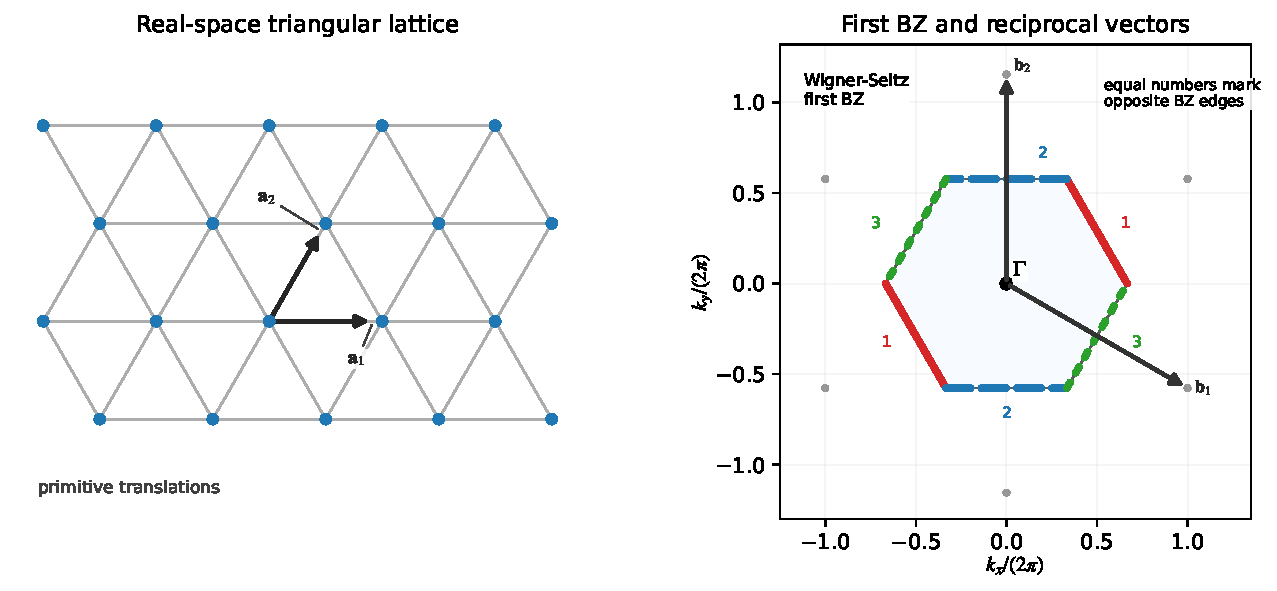
\includegraphics[width=0.88\textwidth]{figures/fig_ch04_bloch_brillouin.pdf}
  \caption{Real-space periodicity and reciprocal-space sewing.  Bloch
  theory replaces translation in the photonic crystal by a cell-periodic
  field on the Brillouin-zone torus; opposite BZ boundaries are identified
  by reciprocal-lattice phase factors, an issue that becomes important in
  numerical Chern computations.}
  \label{fig:ch04-bloch-brillouin}
\end{figure}

\section{Photonic band structure in practice}
\label{sec:ch4-practical-bands}

The Bloch theory and plane-wave expansion method developed in this
chapter provide the foundation for computing photonic band structures.
This section discusses practical aspects of band-structure
calculations that are important for topological photonics
applications.

\subsection{High-symmetry paths and the irreducible Brillouin zone}
\label{sec:ch4-high-symmetry-paths}

Band structures are conventionally plotted along high-symmetry
paths connecting special points of the Brillouin zone.  For the
triangular lattice (the most common lattice in topological photonics),
the standard path is $\Gamma\to M\to K\to\Gamma$, where
$\Gamma=(0,0)$, $M=\bvec_1/2$, and $K=(2\bvec_1+\bvec_2)/3$ in
reciprocal lattice coordinates.

The choice of path determines which band crossings and gaps are
visible in the band diagram.  In particular, Dirac cones at the $K$
and $K'$ points (Chapter~\ref{ch:dirac-cones}) are visible only if
the path passes through these points.  A common mistake is to plot
the band structure along $\Gamma\to X\to M\to\Gamma$ (the path
for a square lattice), which misses the Dirac cones entirely
\cite{press2026photonic,initio2026pdf}.

\subsection{Convergence with respect to plane waves}
\label{sec:ch4-pwe-convergence}

The plane-wave expansion method represents the periodic part of the
Bloch modes as a Fourier series truncated at $|\Gvec|\leq G_{\max}$.
The number of plane waves $N_G$ scales as $G_{\max}^d$ in $d$
dimensions, and the computational cost of diagonalisation scales
as $O(N_G^3)$.  For 2D photonic crystals, convergence of the lowest
bands typically requires $N_G \sim 100$--$500$, corresponding to
$G_{\max} \sim 5$--$10$ reciprocal lattice vectors.

The convergence rate depends on the dielectric contrast
$\varepsilon_{\max}/\varepsilon_{\min}$: higher contrast requires
more plane waves because the field variations are sharper.  For
the YIG photonic crystals of Chapter~\ref{ch:microwave-crystal}
($\varepsilon_{\mathrm{rod}}/\varepsilon_{\mathrm{air}} \approx 15$),
convergence to $<0.1\%$ accuracy in the eigenfrequencies requires
$N_G \gtrsim 300$ \cite{zhao2020first,press2026photonic}.

Figure~\ref{fig:ch04-pwe-convergence} illustrates the two key aspects of the
plane-wave expansion.  Panel~(a) shows the reciprocal-lattice vectors of a
triangular lattice, partitioned into a kept core (blue), an added convergence
shell (orange), and discarded higher-order vectors (grey).  The dashed circles
mark two values of the truncation radius $G_{\max}$; increasing $G_{\max}$
adds more plane waves but raises the matrix dimension.  Panel~(b) shows the
resulting convergence of a representative normalised eigenfrequency
$\omega a/2\pi c$ as the number of plane waves $N_G$ grows from~25
to~441.  The frequency approaches the independently computed reference value
(dotted line) from above, while the relative error (red, right axis,
$\log_{10}$ scale) decreases by more than two orders of magnitude.  In practice,
the discrete $N_G$ values correspond to successive circular truncation shells
of the reciprocal lattice.

\begin{figure}[t]
  \centering
  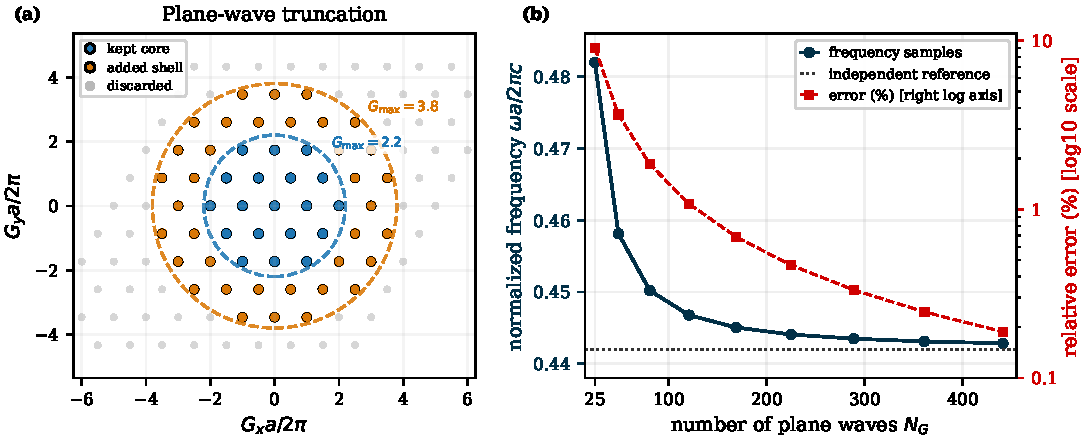
\includegraphics[width=0.95\textwidth]{figures/fig_ch04_pwe_convergence_step178.pdf}
  \caption{Plane-wave expansion in reciprocal space.
  (a)~Reciprocal-lattice vectors of a triangular lattice, classified as kept
  core (blue), added convergence shell (orange), or discarded (grey); dashed
  circles mark two truncation radii $G_{\max}$.
  (b)~Convergence of a normalised eigenfrequency as a function of the number
  of plane waves~$N_G$.  The right axis (red, $\log_{10}$ scale) shows the
  percent relative error with respect to the independently computed reference
  (dotted line).  Each data point corresponds to a successive circular
  truncation shell in reciprocal space.}
  \label{fig:ch04-pwe-convergence}
\end{figure}

\subsection{Supercell method for edge states}
\label{sec:ch4-supercell}

To compute edge-state dispersions, one uses a supercell that is
periodic in one direction (say $x$) and finite in the other ($y$).
The supercell contains a strip of the photonic crystal with the
topological material on one side and vacuum (or a trivially gapped
crystal) on the other.  The edge states appear as bands that cross
the bulk gap.

The supercell width $W$ must be large enough that the edge modes on
opposite boundaries do not hybridise (Section~\ref{sec:ch8-penetration-depth}).
For a topological gap of relative width $\Delta\omega/\omega \sim 3\%$,
a supercell of $\sim 15$--$20$ unit cells in the $y$-direction is
typically sufficient \cite{ozawa2018topological,paz2019tutorial}.

The supercell band structure provides the most direct verification of
the bulk-edge correspondence: one counts the number of edge modes
crossing the gap with positive group velocity and compares with the
bulk Chern number computed from the methods of
Chapter~\ref{ch:computing-chern}.

\section*{Exercises}

\begin{exercise}
  For a 1D photonic crystal (Bragg stack) with alternating layers of
  refractive indices $n_1$ and $n_2$ and thicknesses $d_1$ and $d_2$
  ($d_1+d_2=a$), derive the dispersion relation
  $\cos(ka)=\cos(n_1\omega d_1/c)\cos(n_2\omega d_2/c)
  -\frac{1}{2}(\frac{n_1}{n_2}+\frac{n_2}{n_1})
  \sin(n_1\omega d_1/c)\sin(n_2\omega d_2/c)$
  using the transfer-matrix method.  Identify the band gaps.
\end{exercise}

\begin{exercise}
  Show that the cell-periodic eigenvalue problem \eqref{eq:ch4-cell-evp}
  at $\kvec$ and $\kvec+\Gvec$ are unitarily related:
  $\mathbf{u}_{n,\kvec+\Gvec}(\rvec)
  =\ee^{-\ii\Gvec\cdot\rvec}\mathbf{u}_{n\kvec}(\rvec)$.
  Conclude that the band structure is periodic in $\kvec$.
\end{exercise}

\begin{exercise}
  Derive the Hellmann--Feynman formula \eqref{eq:ch4-hellmann-feynman}
  for the group velocity by differentiating the eigenvalue equation
  with respect to $k_\alpha$ and using the orthonormality of modes.
  Show that in a nondispersive medium the result agrees with the
  energy-velocity formula \eqref{eq:ch4-energy-velocity}.
\end{exercise}

\begin{exercise}
  For the TM modes of a 2D square lattice of circular rods, write out
  the plane-wave expansion matrix \eqref{eq:ch4-pwe-matrix} for the
  case $N_G=9$ (including $\Gvec=\frac{2\pi}{a}(m_1,m_2)$ with
  $m_1,m_2\in\{-1,0,1\}$).  Compute the Fourier coefficient
  $\hat\varepsilon(\Gvec)$ for a circular rod of radius $r$ and
  permittivity $\varepsilon_r$ in a unit cell of side $a$.
\end{exercise}

\begin{exercise}
  At a Dirac point in a hexagonal lattice, the two degenerate modes
  belong to a two-dimensional representation of $C_{3v}$ (the little
  group at $K$).  Using group-theoretic arguments, explain why this
  degeneracy is symmetry-protected and cannot be lifted without
  breaking $C_{3v}$ or time-reversal symmetry.
\end{exercise}
